\chapter{控制系统及仿真模型}

\section{引言}
建立系统的控制模型后,需要考虑模型实现的可能性。
通过分析工作流程, 设计合理的伺服控制方案; 结合系统性质优化PD算法, 用于实现力控。
为验证方案的合理性, 利用Simscape搭建仿真模型, 模拟了操作过程中工具的运动情况。

\section{伺服控制}
本文的研究方案是根据夹持物体当前的运动状态推算夹爪需要施加给物体的正压力,
进而控制物体的运动,因此需要高精准和高频率的力控。
可使用高速相机等设备实时测量被控物体相对于夹爪的位置和速度,对比预先设定的运动状态,
即由式(\ref{equ:2-4})、式(\ref{equ:2-7})反求当前时刻夹爪施加给物体的正压力的期望值。
在这一过程中,我们主要有两个任务,一是不断地获取机器人手的期望位置控制机器人手的运动;
二是周期性地从相机或传感器采集数据,实时地传递给控制系统;
这两个任务的运行周期会有较大差距,因此我们至少需要两个线程来实现这一任务。
此外还需要一个线程处理系统与用户的交互过程。
程序流程图如图\ref{fig:3-1} 所示。

\begin{figure}[!ht]
  \centering
  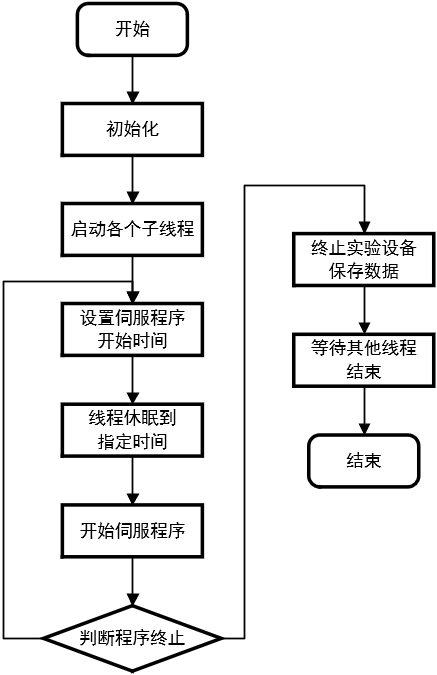
\includegraphics[width=5.5cm]{chapter03/pic/3-1}
  \caption{伺服控制主程序流程图\label{fig:3-1}}
  \vspace{-0.3cm}
\end{figure}

流程图中三个线程分别为伺服线程、交互线程和数据采集线程,
分别处理上文中提到的三个主要任务。各线程间通过一个全局的自定义结构体实现数据互通,
该结构体主要包括夹爪的实际位置、期望位置,系统运行时间,被控物体受力大小、
期望压力值,运动模式标志等数据信息;其作用是实现线程之间的数据共享。
伺服线程即主线程作用是判断当前夹爪的运动状态、实现力控和位置伺服等。
其流程图如图\ref{fig:servo}所示,
该线程中程序首先从全局变量拷贝共享数据结构体到当前函数,
读取夹爪当前位置和系统运行的时间,即获取系统的实时信息。
随后读取压力传感器数据并传入 PD 控制器,得到反馈的位置期望值,并发送控制指令。
最后将这一周期中改变的数据同步到全局变量,同时把权限交由系统分配。

\begin{figure}[!ht]
  \centering
  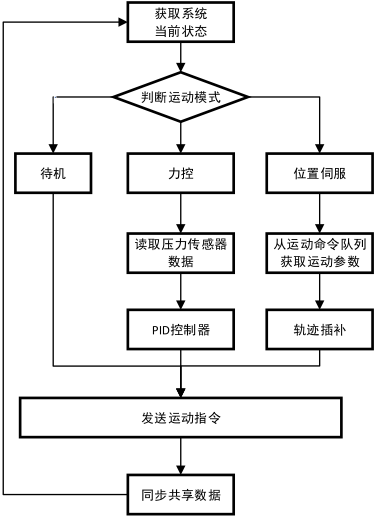
\includegraphics[width=7.5cm]{chapter03/pic/3-2-a}
  \caption{伺服线程的流程图\label{fig:servo}}
  \vspace{-0.3cm}
\end{figure}

% \begin{figure}[!ht]
% \centering
%   \subfloat[]{
%     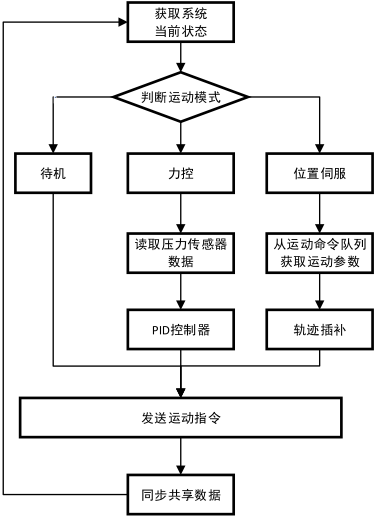
\includegraphics[scale=0.6]{chapter03/pic/3-2-a}
%     }
%     \hspace{25pt}
%   \subfloat[]{
%     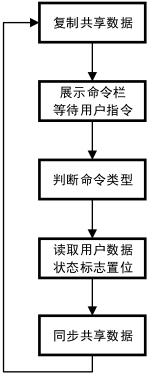
\includegraphics[scale=0.6]{chapter03/pic/3-2-b}
%     }
%     \hspace{25pt}
%   \subfloat[]{
%     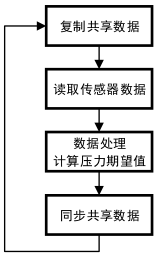
\includegraphics[scale=0.6]{chapter03/pic/3-2-c}
%     }
%   \caption{子线程流程图}
%   \label{fig:3-2}
%   \vspace{-0.3cm}
% \end{figure}

交互线程的作用使处理程序与操作者之间的交互,即一方面将用户输入的命令
和参数传递给系统,另一方面将系统的运行状态等信息展示给用户,
其流程图如图\ref{fig:3-2}a)所示。
进入在该线程后,程序从全局拷贝一份共享数据,以免在运行过程中由于权限被收回而终止线程,
导致各线程之间数据不统一。随后输出菜单栏,等待用户输入指令和运动参数。
根据用户的输入将相应的状态标志置位、更新运动参数,并将参数同步到共享数据,
然后进入下一个循环。

% \begin{figure}[!ht]
%   \centering
%   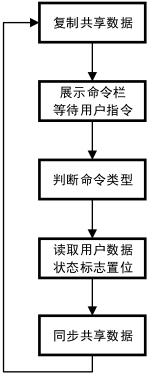
\includegraphics[width=3.5cm]{chapter03/pic/3-2-b}
%   \caption{交互线程的流程图\label{fig:interface}}
%   \vspace{-0.3cm}
% \end{figure}

数据采集线程的主要作用是采集被控物体的运动信息,返回压力期望值。
该线程中工作流程如图\ref{fig:3-2}b)所示, 同样是先从全局拷贝数据;接着读取传感器信息,
计算被控物体的位移和运动速度,根据式(\ref{equ:2-4})得到的期望运动状态计算偏差,
进而根据式(\ref{equ:2-7})得到期望的压力值;在一个周期最后更新共享数据。

\begin{figure}[!ht]
\centering
  \subfloat[交互线程的流程图]{
    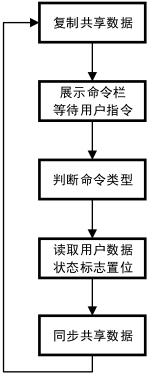
\includegraphics[scale=0.85]{chapter03/pic/3-2-b}
    }
    \hspace{25pt}
  \subfloat[数据采集线程的流程图]{
    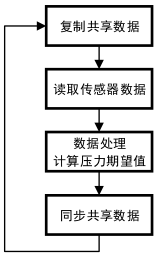
\includegraphics[scale=1]{chapter03/pic/3-2-c}
    }
  \caption{子线程流程图}
  \label{fig:3-2}
  \vspace{-0.3cm}
\end{figure}

% \begin{figure}[!ht]
%   \centering
%   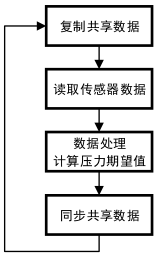
\includegraphics[width=5.5cm]{chapter03/pic/3-2-c}
%   \caption{数据采集与处理线程的流程图\label{fig:collect}}
%   \vspace{-0.3cm}
% \end{figure}



\section{力控研究}
由于我们设计的算法是通过改变施加给工具的正压力来调整工具运动状态,
同时考虑到夹爪和工具的接触模型比较复杂 \cite{ref11} ,
所以使用力控可以降低算法的复杂度,也在一定程度上提高了程序效率。

该控制系统中,前馈量为期望压力值,输出量为夹爪位置,这一控制过程中需
要反馈实际压力大小,我们选择使用传统的 PID 控制。
虽然控制器的选择面很宽泛,但是控制器的选择对我们力控研究的影响不大,
没必要舍弃高效的算法换取微量的精度提升。
而且该系统中对夹具的力控不会产生静差,所以可以舍弃积分项,采用PD控制。
从另一个角度考虑,在实验过程中工具受到的压力变化不大,
夹爪的位移和工具受力可近似视作线性时不变模型,即该系统局部趋于线性,
因此使用 PD控制完全可以满足我们的需求。

我们项目中 PD 控制器的任务是根据压力传感器数据计算的实际压力值调整夹爪位置,
使压力趋于期望值。我们在经典 PD 控制的基础上增加了一些改进策略,
比如引入变控制系数, 添加容差区间等。
经过改进后的PD控制算法流程图如图 \ref{fig:3-3} 所示。

\begin{figure}[!ht]
  \centering
  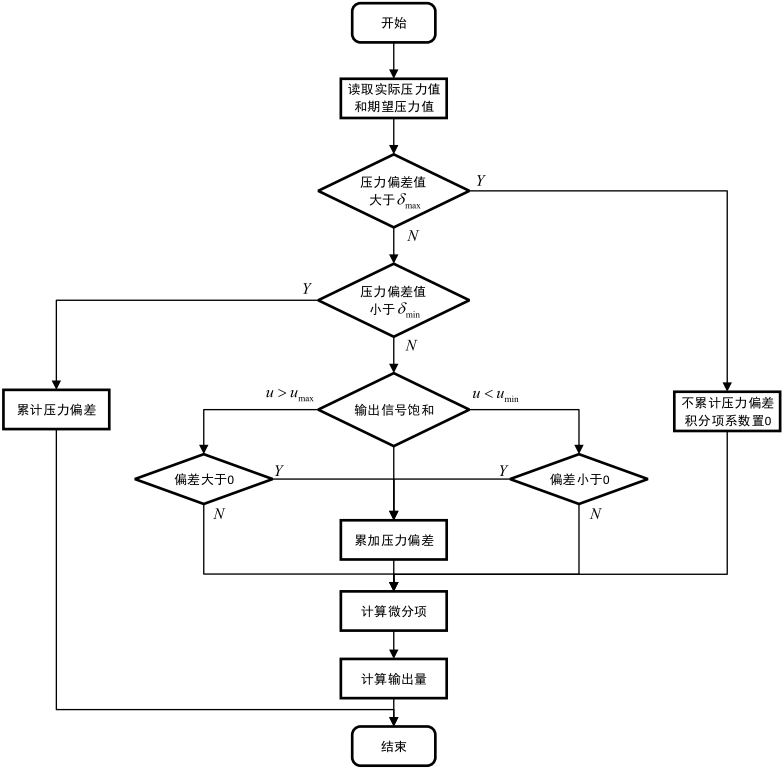
\includegraphics[scale=0.6]{chapter03/pic/3-3}
  \caption{PD控制算法流程图}
  \label{fig:3-3}
  \vspace{-0.3cm}
\end{figure}

引入变比例系数的目的是更好的将系统线性化。
由于我们的传感器采集的电压信号转化为压力信号的过程是非线性的,
通过设计电路后仍然在边缘区域会有较明显的非线性现象。
所以我们在压力信号过小和过大时分别增大和缩小比例系数,
以使得PD控制器在全区间对压力变化的响应相似。
否则在压力过小时系统响应过慢, 调节时间增长;
在压力过大时系统响应过大, 造成压力过大, 系统急停。
而引入变微分系数的目的是防止在误差较大时微分项降低控制输出而使得调节时间增长。
最后由于传感器采集的不稳定性, 控制器获得的输入信号会高频地波动, 为避免夹爪也随之振动,
我们让系统偏差在一定范围内时输出量保持恒定。

\section{仿真的实验设计}
利用 Simscape 可以很方便地搭建机电系统模型。仿真模型可以像装配物理系统一样。
Simscape 采用物理网格法构建模型,模块相当于物理元器件,电机、运算放大器等。
模块之间的连线也类似物理连接,用于传递能量和数据信息,通过这种方法描述的是系统的物理结构,
而非底层的数学原理,所以模型和原理图相似。
此外,Simscape可以从建立的模型中自动构造代数微分方程,描述系统的动态性能。
这些微分方程与Simulink的其他模块集成,直接对微分方程进行求解,
同时求解不同组件的变量,可以有效避免代数环的问题。

为了简单验证该方案的可行性,我们选择建立仿真模型来模拟机器人手操作工具的过程。
我们在 Simulink 的多体动力学模块(Simscape Multibody)中,搭建了系统仿真模型,
包括了实际的物理系统和上文设计好的控制系统,并进行仿真实验。
模拟了操作过程中工具的运动情况,以验证了控制算法的准确性。

\begin{figure}[!ht]
  \centering
  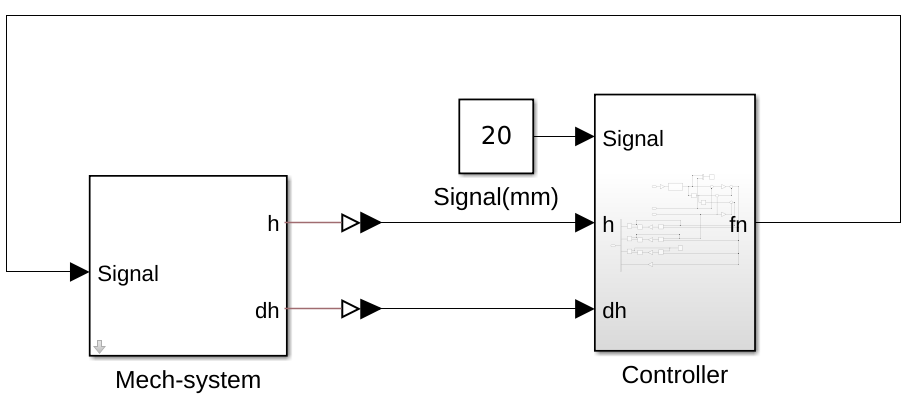
\includegraphics[scale=0.60]{chapter03/pic/3-4}
  \caption{Simulink仿真模型图}
  \label{fig:3-4}
  \vspace{-0.3cm}
\end{figure}

该 Simulink 模型如图 \ref{fig:3-4} 所示,共分为两个子系统:
物理模型统子系统和控制器子系统。
物理模型中可以模拟机械结构的运动状态,同时模拟相机和传感器等设备,
实时测量工具的位置、速度和加速度,并发送到控制器。
控制器则根据接收到的信号在线调整控制系统结构参数,
并且计算夹爪需要施加给工具的正压力,以指令的形式发送到机械系统子模块,
控制夹爪和工具的运动。

机械系统子模块的模型图如图 \ref{fig:3-5} 所示。
该模块中工具(Bar)能在重力作用下自由运动,
其运动的位置、速度和加速度为该子系统输出,反馈到控制系统。
Gripper-L,Gripper-R 为夹爪的两个手指,
分别与工具之间设有接触模块,以模拟夹具与工具之间的接触情况。
假定右手指静止,左手指仅有一个横向运动自由度,
通过左手指的运动给工具施加压力产生摩擦。
这一接触模型中,我们假设了物体间的形变量与弹性力成正比,即刚度系数为常数。

\begin{figure}[!ht]
  \centering
  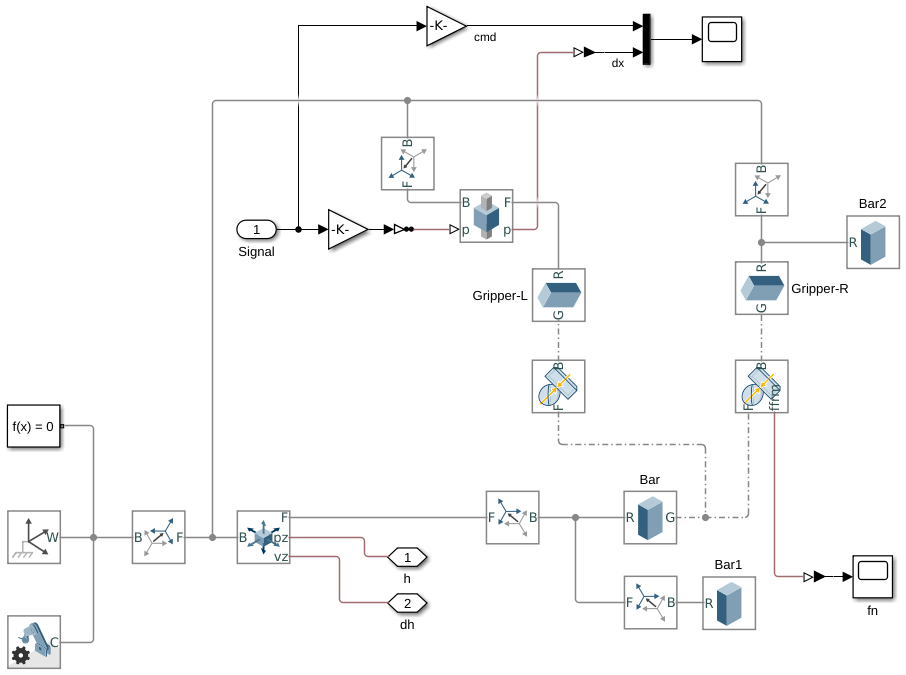
\includegraphics[scale=0.6]{chapter03/pic/3-5}
  \caption{物理模型子系统}
  \label{fig:3-5}
  \vspace{-0.3cm}
\end{figure}

控制器子模块的结构如图 \ref{fig:3-6} 所示。子系统输入中 $Signal$ 为工具的目标位置,
$h$ 、$dh$ 分别为物体当前时刻的位置和速度;
输出 $f_n$ 为夹爪应该施加给工具的正压力信号,
该信号由模型参考自适应控制方程计算得到。
该子系统首先根据式(\ref{equ:2-4})计算物体当前时刻的运动状态,
和机械系统子模块反馈的实际运动状态对比,计算得到当前状态误差。
随后,根据式(\ref{equ:2-7})计算出需要施加给工具的正压力,
并发送给机械系统子模块,为夹爪提供期望的压力值。
进一步地,控制系统在循环中不断地根据式(\ref{equ:2-8})调整控制系统结构参数;
以使得工具的运动状态与期望状态的广义误差$s$收敛到0。

\begin{figure}[!ht]
  \centering
  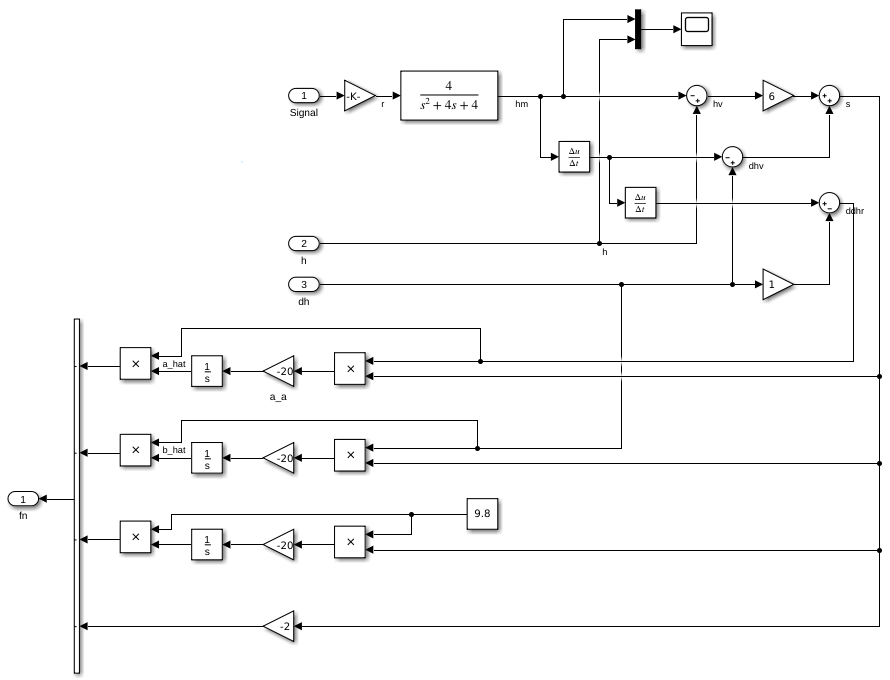
\includegraphics[scale=0.55]{chapter03/pic/3-6}
  \caption{控制模型子系统}
  \label{fig:3-6}
  \vspace{-0.3cm}
\end{figure}

\section{仿真实验}
为验证上文提出的想法的可行性,我们设计了仿真实验。
采用表 4-1 所示的物理参数带入图\ref{fig:3-5}所示的 Simulink 模型中进行仿真实验,
观察实验现象并分析仿真结果与实验结果的差距和原因。虽然仿真实验中数据可能会过于理想,
但是这在某种程度上也能佐证方案的合理性。
在这次仿真试验中,我们通过直接给夹爪运动副施加控制力,即力控是理想的。
这样可以证明我们推导的动力学模型和控制模型理论上是正确的。

\begin{table}[!h]
\centering
\caption{仿真实验参数取值表\label{tab:4-1}}
\begin{tabular}{@{}ccccccccc@{}}
\toprule[1pt]
 \makebox[3.5em][c]{$h_d/mm$}   & \makebox[2.5em][c]{$m/g$}  &
 \makebox[2.5em][c]{$\mu$}      & \makebox[2.5em][c]{$\sigma$}  &
 \makebox[2.5em][c]{$k$}        & \makebox[2.5em][c]{$\lambda$}  &
 \makebox[2.5em][c]{$\alpha_a$} & \makebox[2.5em][c]{$\alpha_c$}  &
 \makebox[2.5em][c]{$\alpha_c$} \\ \midrule

20       &  12       &  0.5     &  0.3    &2        &  6        &
20      &  20     &  20    \\
\bottomrule[1pt]
\end{tabular}
\end{table}


工具下落过程中的位置变化曲线如图 \ref{fig:4-7} 所示。从图中可以看出,工具的位移
曲线很好地跟随了参考模型信号,并且最终停在了目标位置 $h = 20 mm$ 处。由此可
知,模型参考自适应控制系统能够达到理想的控制效果,本次实验中在并未给出具
体的摩擦参数以及物体质量的情况下,平行指夹具仍然成功地控制工具运动到了目
标位置。


\begin{figure}[!ht]
  \centering
  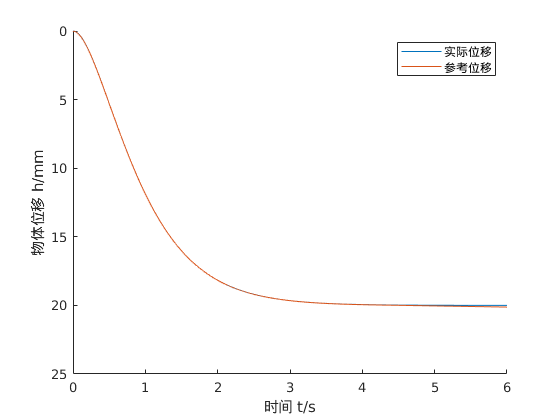
\includegraphics[width=11cm]{chapter04/pic/h_f}
  \caption{工具位移曲线}
  \label{fig:4-7}
  \vspace{-0.3cm}
\end{figure}


夹具位置信号的变化曲线如图 \ref{fig:p_f} 所示。图中 t = 0 s 附近,
即仿真刚开始时的一小段突变是由于初始状态下夹具与工具之间并未紧密接触,
工具的快速下落与参考模型中的输出信号的广义偏差很大,所以夹具位移突变很大。
时间在0s 到 2s左右夹具位置几乎无变化, 这是因为在这段时间内夹具的运动可近似为匀速运动,
而在0s左右时,控制器已经通过实时的广义误差估计出了摩擦系数,
所以这段时间内夹具只需要保持在固定位置即可实现工具的匀速运动。
时间在 2s 到 2.5s 附近夹具位置变化频繁,
这是因为工具速度发生变化,运动过程中需要保持工具运动曲线跟踪参考曲线,所以夹具运动频繁。
另一方面,由于该仿真模型中夹具和工具都接近刚体,导致两模型的碰撞效果明显。
在 3s 之后,夹具位置变化趋于稳定,说明工具运动减慢,并逐渐停止。
由于存在少许的超调量,广义误差 s 一直小于零,所以压力应该持续增大,导致夹具位移持续增大。

% \begin{figure}[!ht]
%   \centering
%   \includegraphics[scale=0.6]{chapter04/pic/4-8}
%   \caption{夹具位移曲线}
%   \label{fig:4-8}
%   \vspace{-0.3cm}
% \end{figure}

压力传感器记录的数据如图 \ref{fig:fn_f} 所示。压力的变化趋势与夹具位移一致,
这是因为接触模型中形变量与弹性力成正比。
为了更好的仿真效果,需要修正夹具模型,将其修改为刚度系数较小的弹性体。

\begin{figure}[!ht]
  \centering
  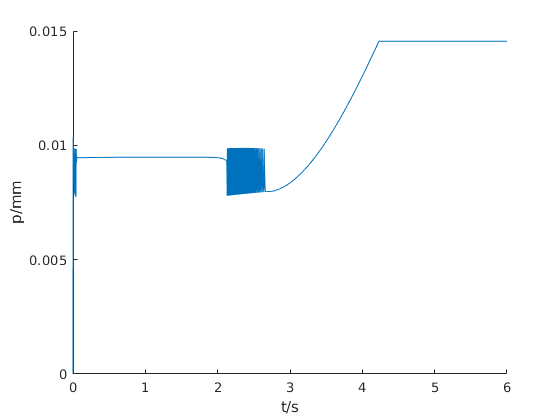
\includegraphics[width=10.2cm]{chapter04/pic/p_f}
  \caption{\label{fig:p_f}
    仿真实验中夹具位移曲线图}
  \vspace{-0.3cm}
\end{figure}

\begin{figure}[!ht]
  \centering
  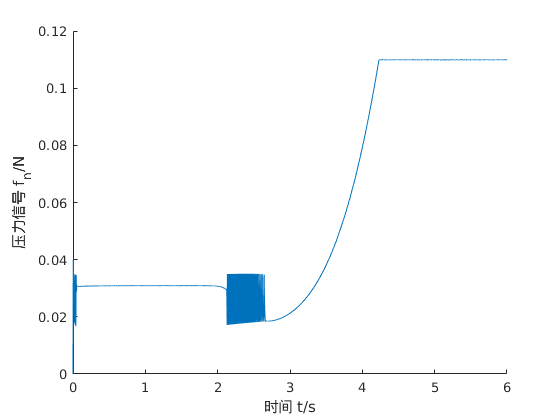
\includegraphics[width=10.2cm]{chapter04/pic/fn_f}
  \caption{\label{fig:fn_f}
    仿真实验中物体所受压力曲线}
  \vspace{-0.3cm}
\end{figure}

% \begin{figure}[!h]
%   \centering
%     \subfloat[夹具位移曲线]{
%       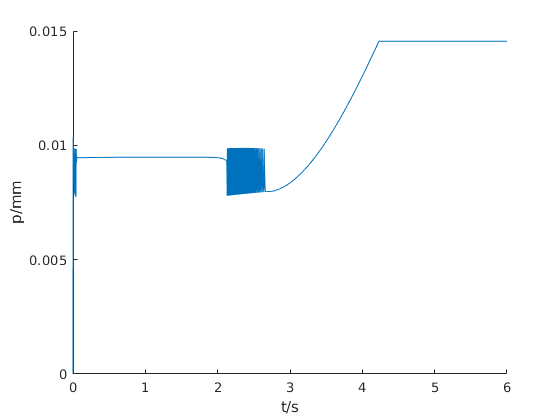
\includegraphics[width=7.2cm]{chapter04/pic/p_f}
%     }
%     \hspace{0pt}
%     \subfloat[压力变化曲线]{
%       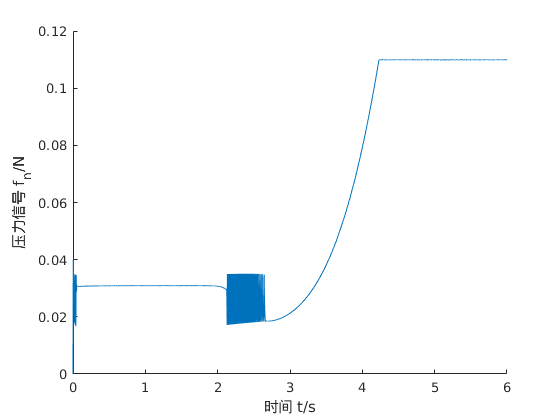
\includegraphics[width=7.2cm]{chapter04/pic/fn_f}
%     }
%   \caption{夹具位移及受力曲线图}
%   \label{fig:4-8}
%   \vspace{-0.3cm}
% \end{figure}

通过这一仿真实验,我们可以确保上文推导的工具动力学方程(式 \ref{equ:2-3})的正确性,
以及适应性控制方程(\ref{equ:2-7})和调参规律(\ref{equ:2-8})可以保证跟踪误差的收敛,
可以精准控制物体下落的轨迹。


\section{添加力控的仿真实验}
在实际实验过程中,理想的力控是难以实现的。
为了更好的仿真效果, 我们需要修改仿真模型,
我们在图 \ref{fig:3-5} 的基础上为夹爪添加了一个弹簧模型, 以模拟实际场景中的缓冲垫片。
并且直接对运动副施加控制力的方案被修改为对运动副施加位移控制,
以模拟控制器对夹爪发送的控制指令。
然后添加PD控制子模块, 并调整合适的参数,以模拟真实场景中的力控效果。
最终机械系统子模块的仿真模型图如下图 \ref{fig:mech_x} 所示。

\begin{figure}[!ht]
  \centering
  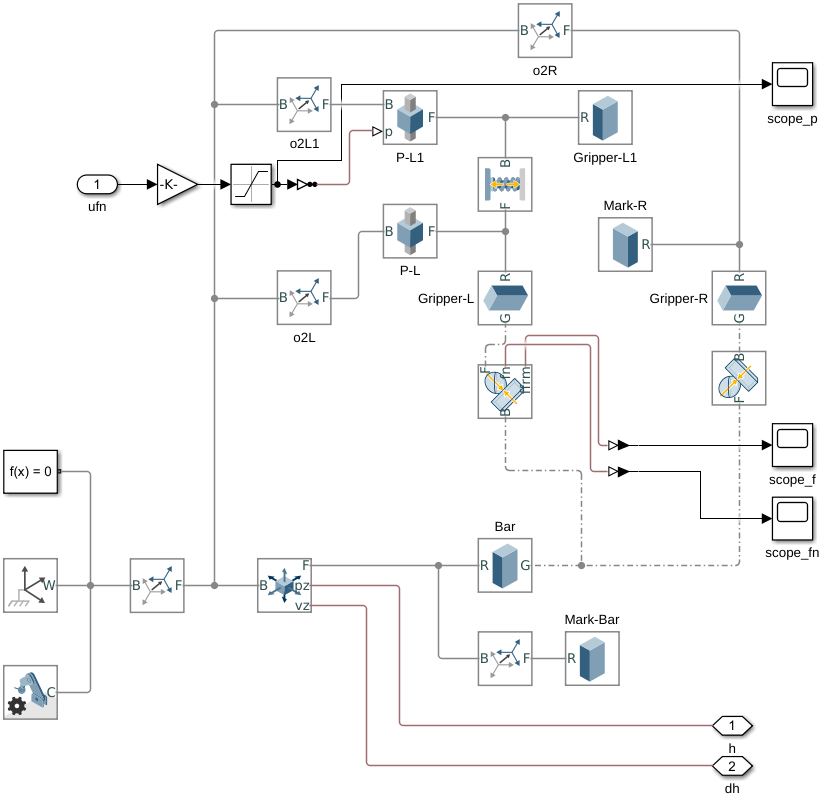
\includegraphics[width=13.5cm]{chapter04/pic/mech_x}
  \caption{\label{fig:mech_x}
    添加力控的机械系统模块}
  \vspace{-0.3cm}
\end{figure}

再次重复上述实验, 工具的位移曲线如 \ref{fig:h_x} 所示。
从图中可以看出,工具的位移曲线依旧能跟随了参考模型信号,
虽然会出现频繁停止和突然运动的现象,但是工具最终依然停在了目标位置 $h = 20 mm$ 处。
由此可知, 我们使用的控制方案能够达到理想的控制效果。
但是这次实验中也暴露出一些问题, 比如在快达到目标位置但还未达到时,
控制器会累计误差, 直到误差足够大时, 夹爪会张开让工具开始运动,
如果夹爪速度不够快或者控制器响应速度不够高, 那么工具有可能会超过期望位置后才被停止。
这一问题显然可以通过加快系统响应速度来解决, 另一方面, 也可以通过添加一容差区间来解决。
比如让控制器检测到广义误差小到可接受范围内时, 即认为工具已经达到目标位置, 操作结束。
图中工具运动会突然停止再突然运动,这是因为软指接触中,手指上的垫片过软。
由于缓冲效果明显,压力传感器检测到的力变化幅度较小,手指慢慢张开后工具开始下落;
而检测到广义误差过大后,控制器发送指令让手指闭合,手指闭合过程对工具的力被缓和,
工具在手指闭合到既定位置时还能下落一定距离。
这将使得自适应控制器错误的将摩擦系数估计得过小。
因此在下次张开手指时,控制器计算的夹具位移应该比理论值更小, 也使得工具停止时间增长。
另一方面,这也导致了夹具位置变化频繁,
以此保证工具连续运动过程中工具运动曲线能更好的跟踪参考曲线。

\begin{figure}[!ht]
  \centering
  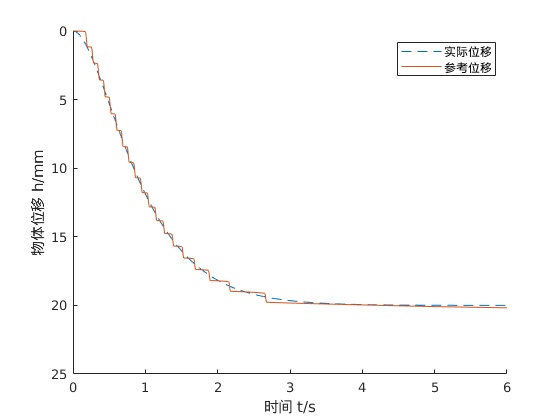
\includegraphics[width=9.7cm]{chapter04/pic/h_x}
  \caption{\label{fig:h_x}
    力控仿真实验中工具位移曲线}
  \vspace{-0.3cm}
\end{figure}


夹具位置信号的变化曲线如图 \ref{fig:p_x} 所示。
图中夹具位置变化频繁,这是由于工具不连续的运动状态导致的,
运动过程中需要保持工具运动曲线跟踪参考曲线,所以夹具运动频繁。
在我们的实验中,我们发现了夹爪手指垫片的刚度系数和工具运动连续程度的定性关系。
当垫片或胶皮过软,即刚度系数过小时,工具每次停止的时间越长,每段下落距离越长,
在工具位移曲线图上表现为阶梯状越明显。
反之运动越连续, 运动曲线对参考曲线的跟踪性能越好。
这并不难理解, 刚度越低时夹具要使工具开始运动或停止运动需要产生的位移越大,
在其他条件如夹具运动速度,PD控制系数等参数相同的情况下, 工具对夹具位移的响应越慢,
因此运动会断断续续, 而且每段运动过程中下落和停止的时间均会增长。
但是, 刚度也不能过高, 因为这需要系统具有更快的响应速度和更精准的力控。
否则可能造成系统震荡, 或夹爪由于受力过大而保护性停止。

\begin{figure}[!ht]
  \centering
  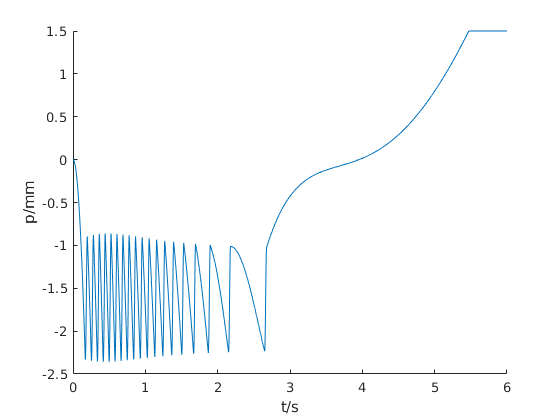
\includegraphics[width=9.7cm]{chapter04/pic/p_x}
  \caption{\label{fig:p_x}
    力控仿真实验中夹具位移曲线}
  \vspace{-0.3cm}
\end{figure}

\begin{figure}[!ht]
  \centering
  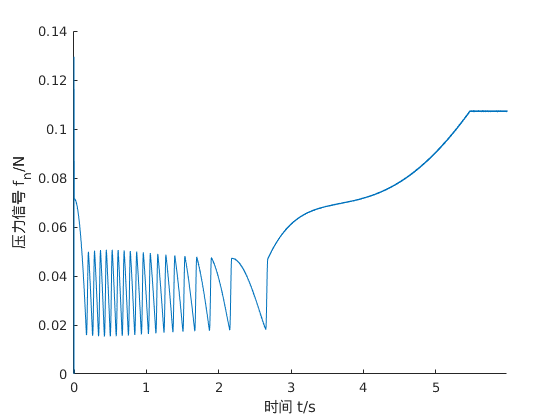
\includegraphics[width=9.7cm]{chapter04/pic/fn_x}
  \caption{\label{fig:fn_x}
    力控仿真实验中物体所受压力曲线}
  \vspace{-0.3cm}
\end{figure}

% \begin{figure}[!h]
%   \centering
%     \subfloat[夹具位移曲线]{
%       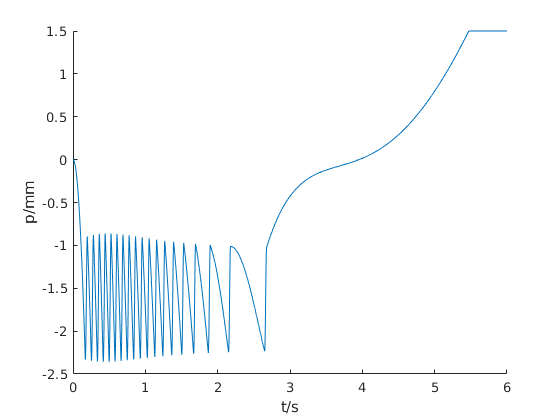
\includegraphics[width=7.2cm]{chapter04/pic/p_x}
%     }
%     \hspace{0pt}
%     \subfloat[压力变化曲线]{
%       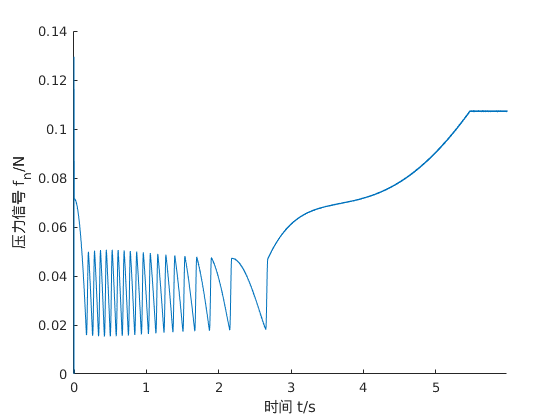
\includegraphics[width=7.2cm]{chapter04/pic/fn_x}
%     }
%   \caption{夹具位移及受力曲线图}
%   \label{fig:4-11}
%   \vspace{-0.3cm}
% \end{figure}

同样,如图\ref{fig:fn_x}在这次实验中夹具施加给物体的压力也会在物体停止后持续增大。
这也由于超调量使得广义误差大于零且一直累加导致的。
为了防止位移信号持续增大而使得信号超过阈值造成机器停止等问题,
我们人为添加了饱和模块,以限制输出的位置指令。

\section{本章小结}
考虑了实际实验过程中可能会遇到的多线程问题,提出了一个合理的方案。
根据实际情况设计了用于进行力控的优化的 PD 控制器。
最后根据系统动力学模型和自适应控制模型,
在 Matlab/Simulink 的多体动力学模块搭建了仿真模型,
可以模拟系统的运动过程和控制回路。

